\newpage
\section{Aplikacja mobilna - kontroler}

\begin{center}
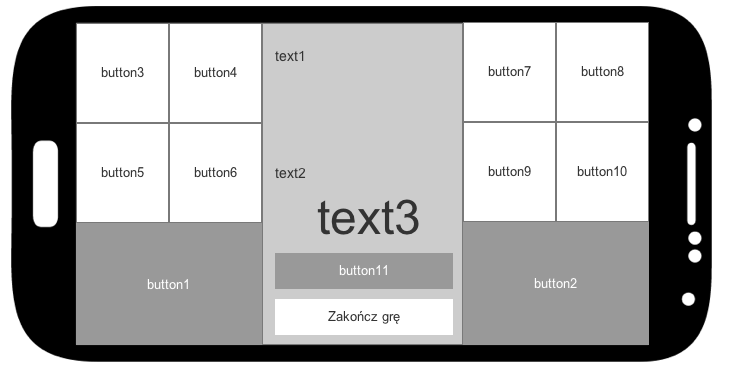
\includegraphics[width=1\textwidth]{images/button_mockup.png}
\captionof{figure}{
Makieta - układ przycisków
}
\end{center}
\paragraph{}
Głównym założeniem było stworzenie uniwersalnego kontrolera przygotowanego pod dowolny rodzaj gry, bądź innej wizualizacji stworzonej w środowisku Unity. Podczas uruchomienia kontrolera serwer wysyła statusy przycisków oraz pól tekstowych.


\begin{center}
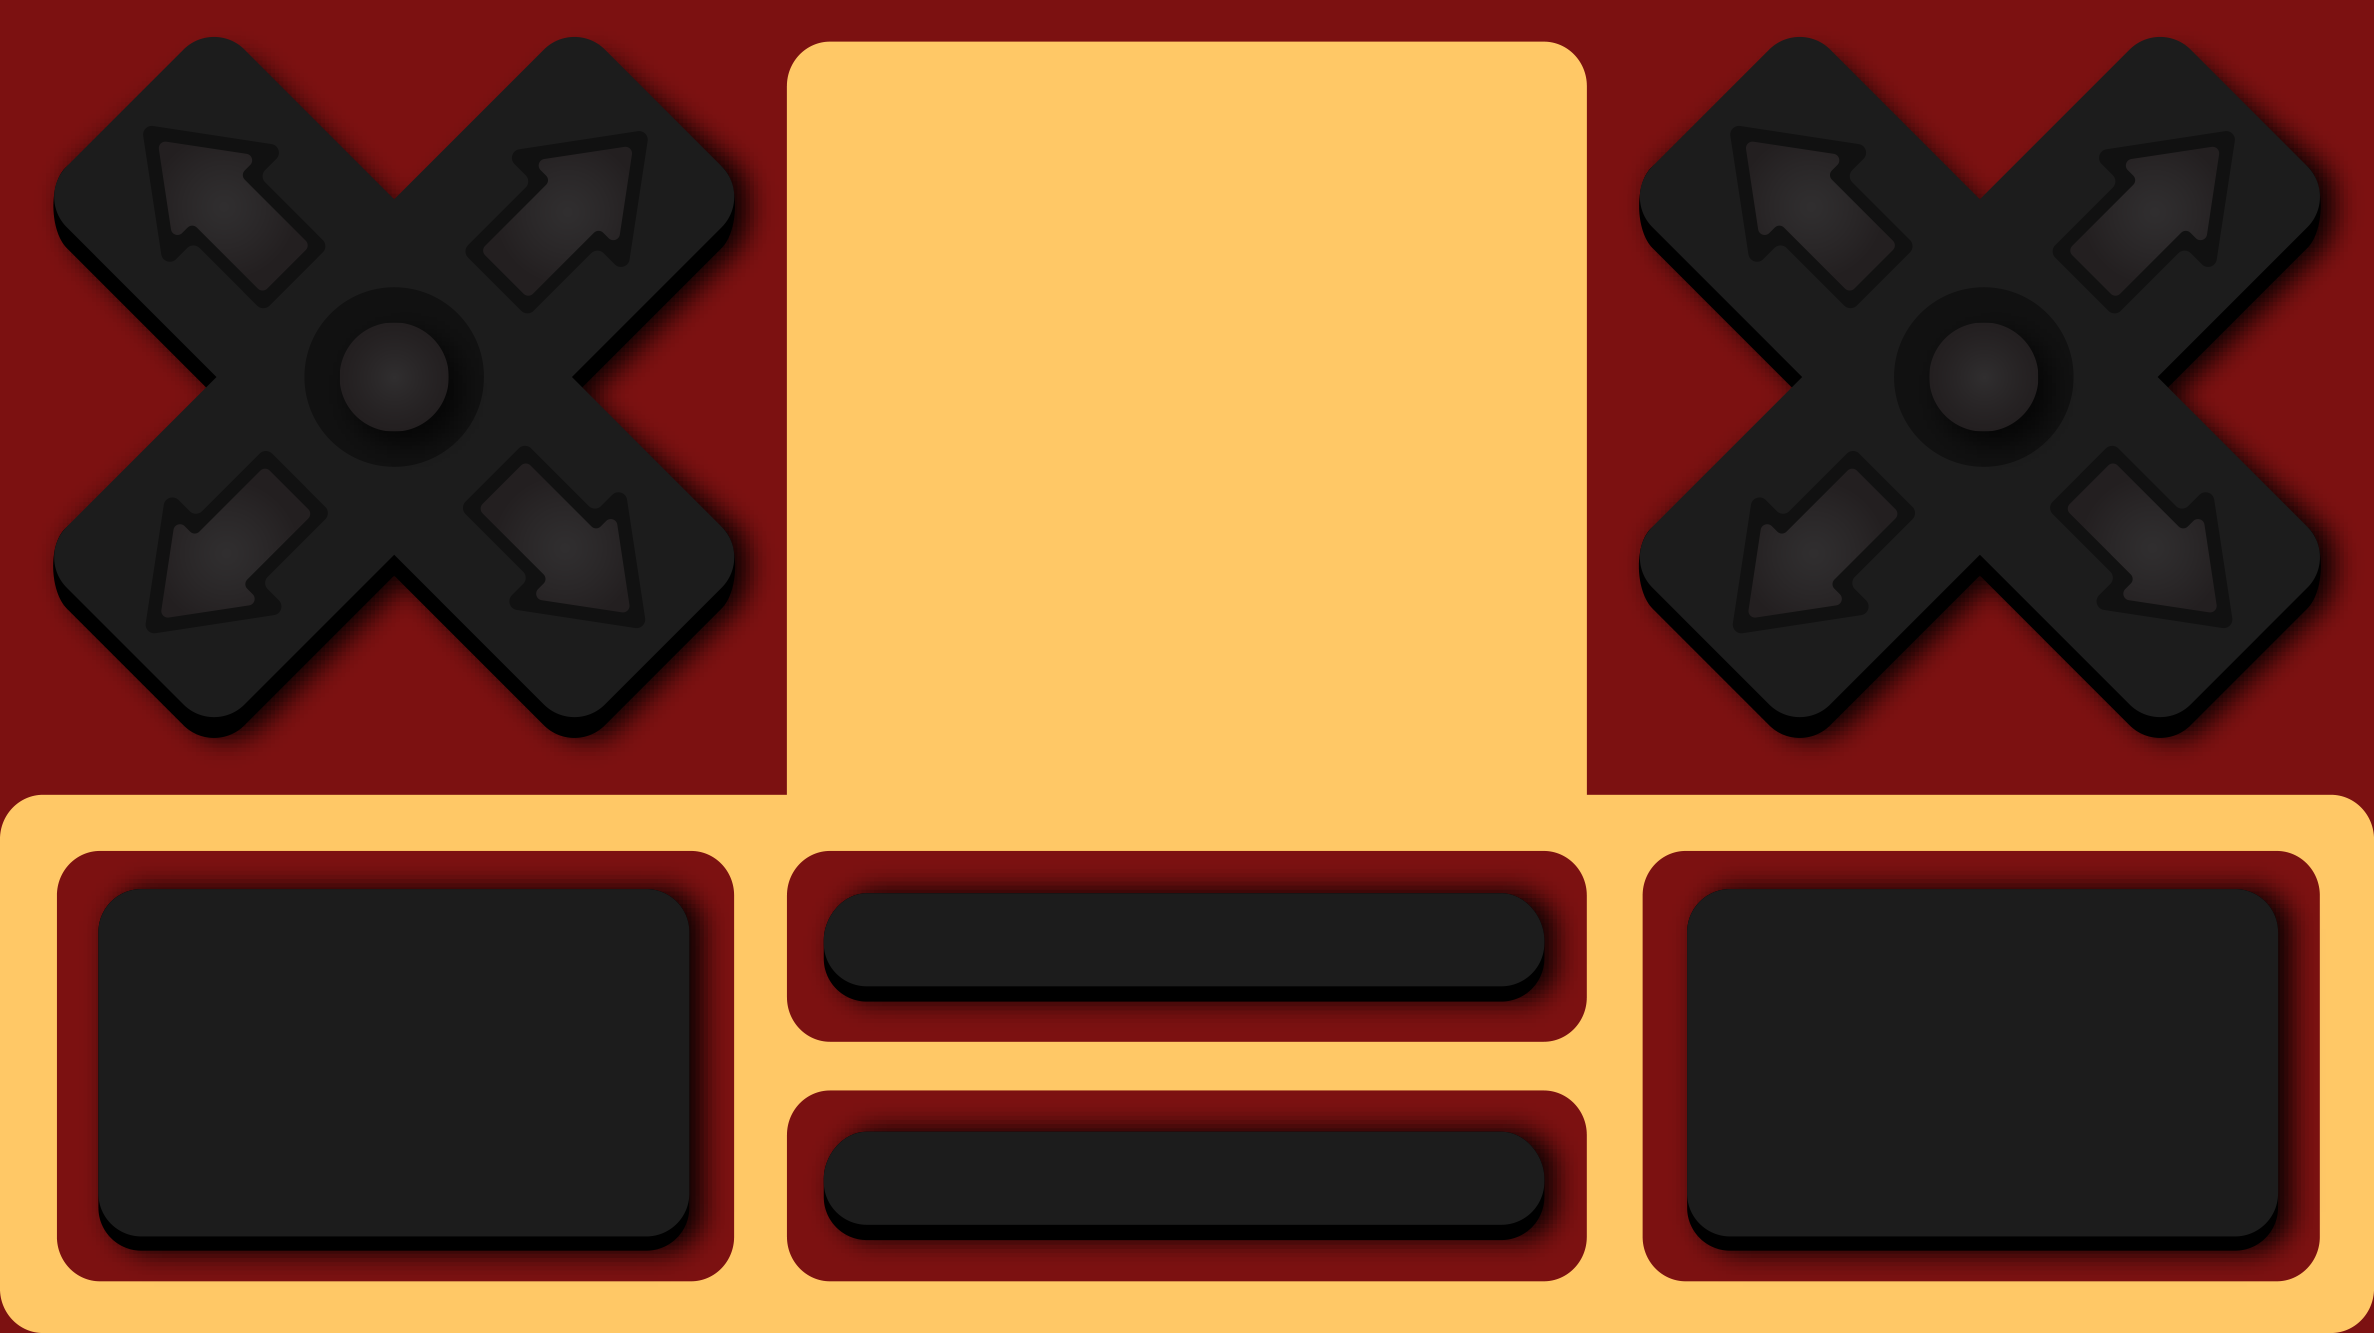
\includegraphics[width=1\textwidth]{images/graph1.png}

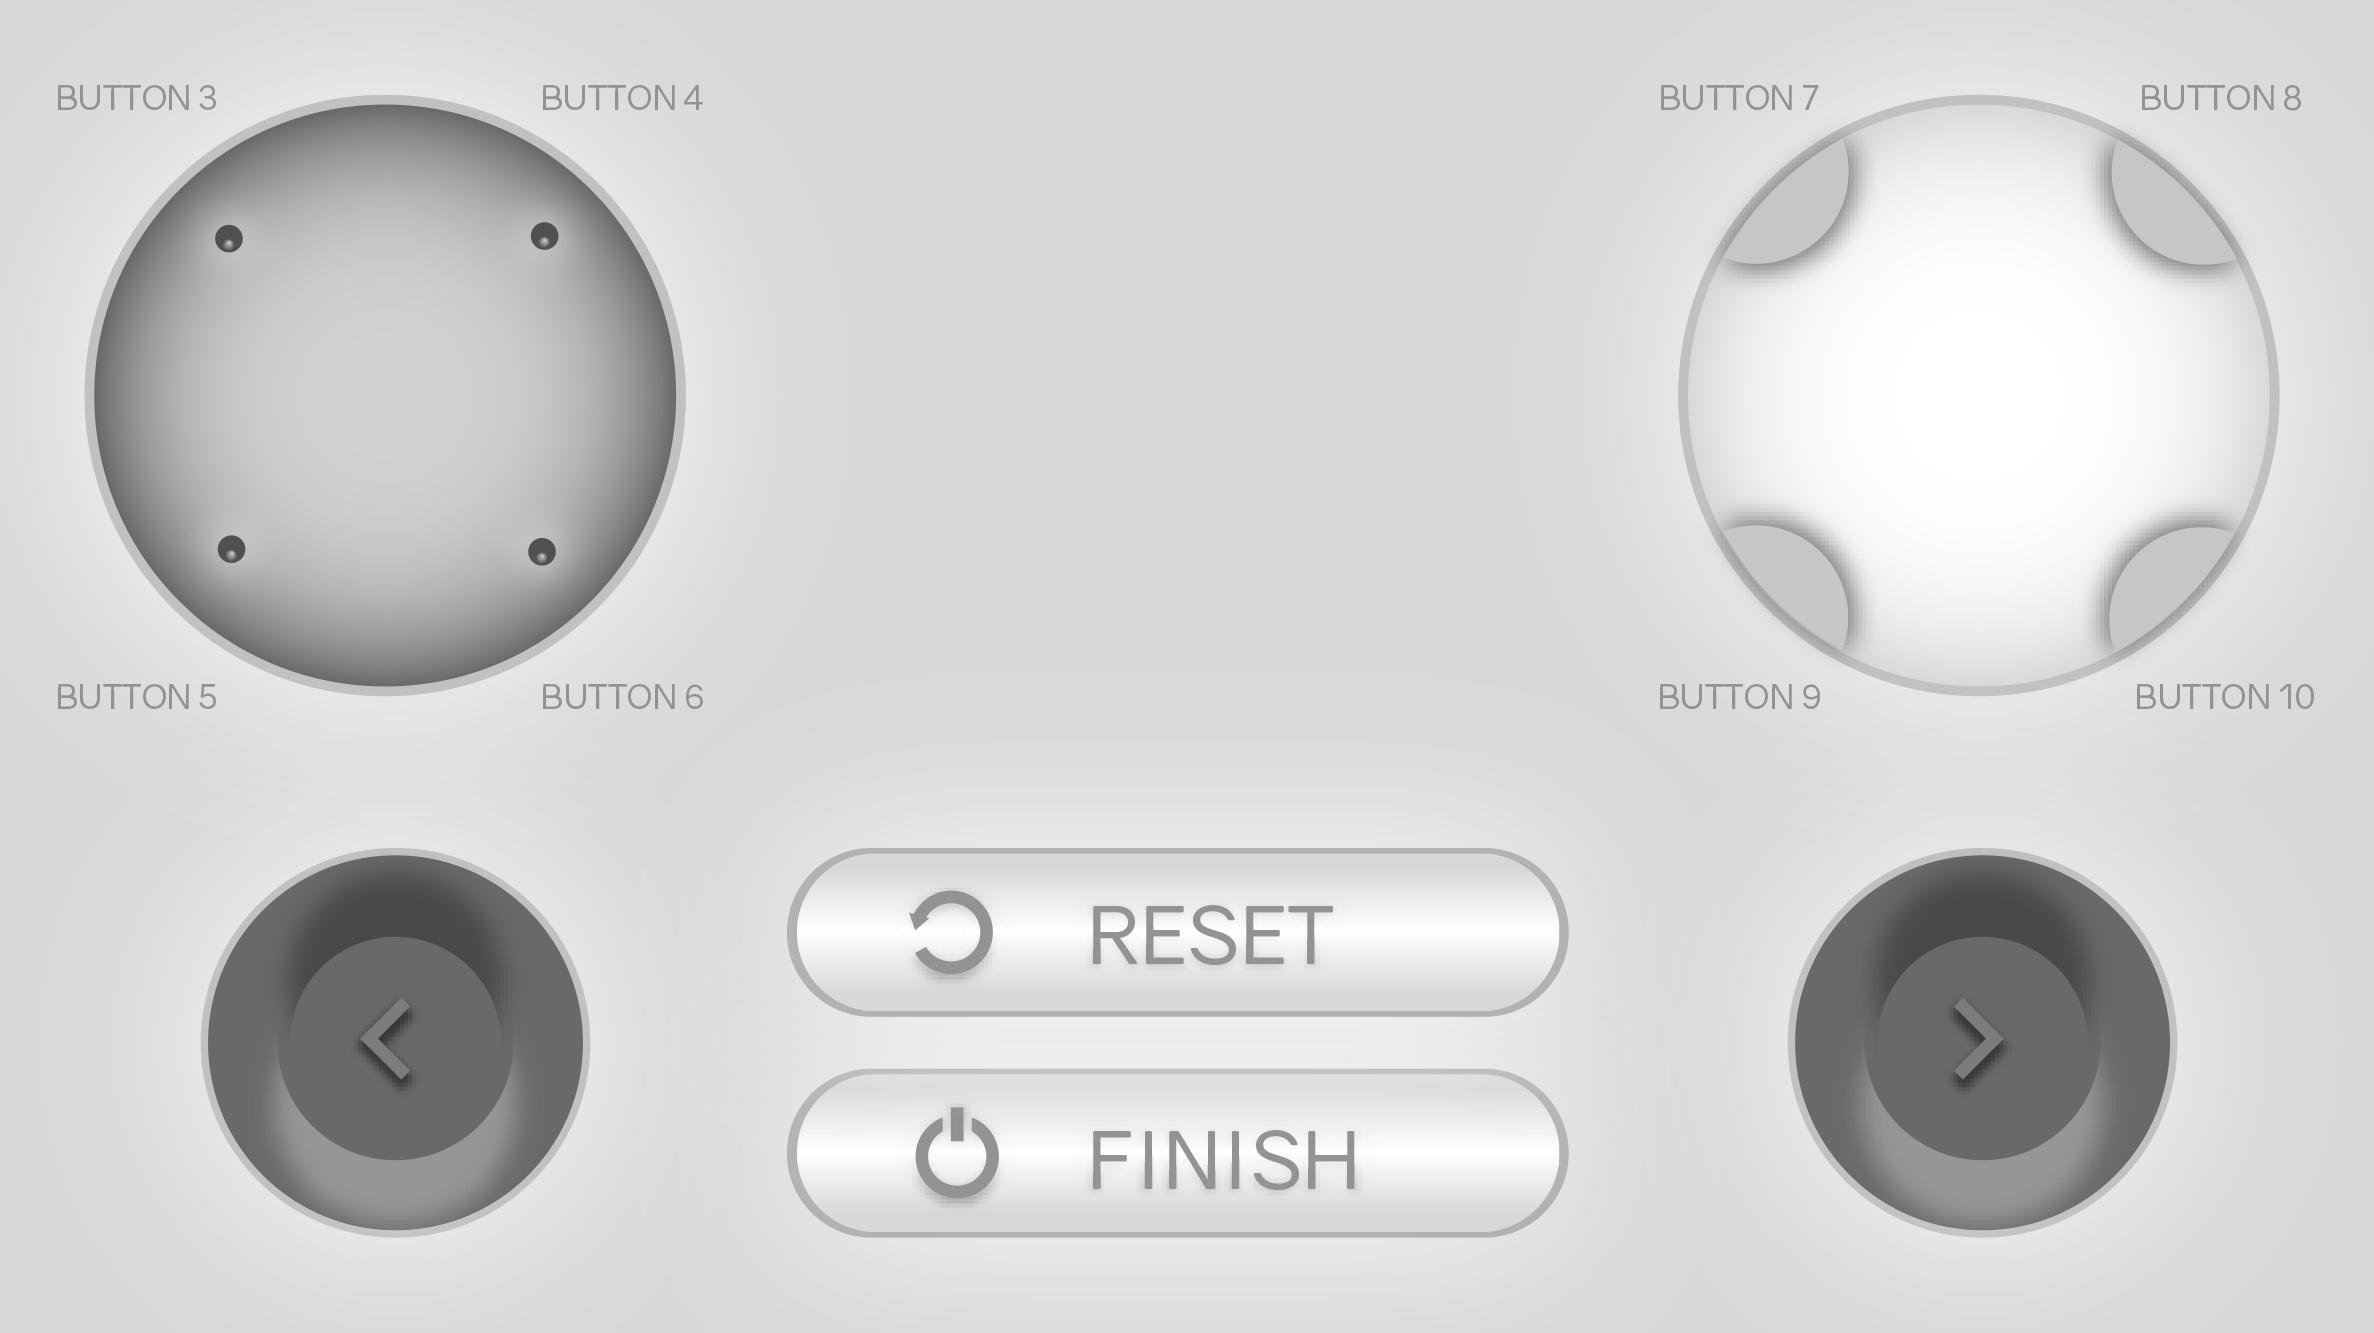
\includegraphics[width=1\textwidth]{images/graph2.png}
\captionof{figure}{
Przykładowa wizualizacja kontrolera
}
\end{center}

\subsection{Przyciski}
\paragraph{}
Każdy przycisk może zostać skonfigurowany poprzez ustawienie tekstu. Dodatkowo można zablokować przycisk podczas gdy nie jest on potrzebny w danym czasie. 
Jednym z główny założeń architektonicznych był rozdzielenie warstwy widoku od logiki biznesowej. Ustalono, że stworzenie nowego przycisku odbywać się będzie wymagało tylko dodania definicji w warstwie widoku (plik layout w formacie XML).

\begin{lstlisting}[language=XML]
<pl.pjatk.remotecontroller.CustomButton
    app:name="button2"
    android:layout_gravity="center_horizontal"
    android:layout_height="wrap_content"
    android:layout_width="wrap_content"
/>
\end{lstlisting}
\captionof{lstlisting}{
	Przykład zdefiniowanego przycisku
}
\paragraph{}
Na potrzeby realizacji powyższego założenia stworzono klasę CustomButton, która jest rozszerzeniem (dziedziczy bezpośrednio) klasy Button znajdującej się w pakiecie  android.widget.
\paragraph{}
Każdy z przycisków musi posiadać własną nazwę kodową, gdyż serwer podczas komunikacji sieciowej identyfikuje przycisk poprzez unikalny klucz. Domyślnie w środowisku Android każdy komponent wizualny może posiadać swoje Id, jednakże jest one reprezentowane poprzez liczbę typu Integer.
Dla ułatwienia dalszego rozwoju aplikacji postanowiono stworzyć nowy atrybut. Ich definicje umieszczas ię w formacie XML w pliku attrs.xml.

\begin{lstlisting}[language=XML]
<resources>
    <declare-styleable name="CustomButton">
        <attr name="name" format="string" />
    </declare-styleable>
</resources>
\end{lstlisting}
\captionof{lstlisting}{
    Definicja atrybutu o nazwie name
}

\paragraph{}
W konstruktorze poza domyślnymi wywołaniami klasy bazowej \texttt{Button} zapisywana jest wartość atrybutu name do zmiennej o tej nazwie oraz następuje wstępna konfiguracja przycisku.

\begin{lstlisting}[language=Java]
private static HashMap<String, CustomButton> buttons = new HashMap<String, CustomButton>();

 private void setUp() {
        buttons.put(getName(), this);
        setText(getName());

        setOnClickListener(new View.OnClickListener(){
            @Override
            public void onClick(View v) {
                ServerCommunication.click_button(getName());
            }
        });

    }
\end{lstlisting}
\captionof{lstlisting}{
    Konfiguracja w klasie CustomButton
}

\paragraph{}
Dzięki metodzie \texttt{setUp} konfigurowany jest przycisk. Ustawiana jest nazwa przycisku (zmiana możliwa za pomocą aplikacji Unity), przycisk jest zapisywany do listy wszystkich dostępych przycisków (dzięki temu konfiguracja ilośći przycisków odbywa się tylko w jednym miejscu - na poziomie warstwy widoku) oraz uruchamiany jest listener. Przy każdym kliknięciu wywułuje się metoda w singletonie \texttt{SerwerCommunication}.


\subsection{Użycie styli}
\paragraph{}
Dodatkowym wymaganiem było umożliwienie szybkiej zmiany wyglądu przycisków w trakcie działania aplikacji. Użycie natywnych styli niestety nie jest możliwe bez ponownego renderowania widoku. Aby zaoszczędzić czas i moc obliczeniową postanowiono, iż zostatnie użyta technologia zmiany tła za pomocą metody \texttt{backgroundResource}. Różne wyglądy przycisku mogą być definiowane jako selektory (zewnętrzne pliki xml w katalogu drawable). Ważne, by plik był odpowiednio nazwany, gdyż po nazwie następuje wyszukiwanie schematu podczas zmiany wyglądu.

\begin{lstlisting}[language=Xml]
<?xml version="1.0" encoding="utf-8"?>
<selector 
xmlns:android="http://schemas.android.com/apk/res/android
">
    <item android:state_pressed="true" >
        <shape>
            <gradient
                android:startColor="#bf1d00"
                android:endColor="#801300"
                android:angle="270" />
            <corners android:radius="10dp" />
            <stroke
                android:width="1dp"
                android:color="#71c2eb" />
        </shape>
    </item>
    <item>
        <shape 
xmlns:android="http://schemas.android.com/apk/res/android"
        android:shape="rectangle">
            <gradient android:startColor="#FFFFFF"
                android:endColor="#999"
                android:angle="270" />
        </shape>
    </item>
</selector>
\end{lstlisting}
\captionof{lstlisting}{
    Przykład zdefiniowanego tła
}
\paragraph{}
Wymaganiem była jednoczesna zmiana wyglądu wszystkich przycisków. Rozwiązano to za pomocą metody statycznej, która iteruje po wszystkich przyciskach i wywołuje metdę \texttt{backgroundResource}.


\begin{lstlisting}[language=Java]
 public static void setLayout(int i) {
    for (CustomButton btn : buttons.values()) {
        btn.setBackgroundResource(i);
    }
}
\end{lstlisting}
\captionof{lstlisting}{
   Zmiana tła dla wszystkich przcisków
}


\begin{lstlisting}[language=Java]
CustomButton.setLayout(R.drawable.dark);
\end{lstlisting}
\captionof{lstlisting}{
   Przykład wywołania zmiany tła przycisków
}

\subsection{Komunikacja sieciowa}

\begin{lstlisting}[language=Java]
public  class ServerCommunication {
    private static Socket mSocket = null;
    private static AppCompatActivity activity = null;

    public static void start(AppCompatActivity mainActivity) {
        activity = mainActivity;
        ServerCommunication.start();
    }

    private static void start() {
        if(mSocket == null) {
            Log.i("socket", "createServer");
            try {
                mSocket = IO.socket("http://192.168.0.12:5555");
                mSocket.connect();
                ServerCommunication.listenDisableButton();
                ServerCommunication.listenEnableButton();
                ServerCommunication.listenSetText();
                mSocket.emit("register_controller");
            } catch (URISyntaxException e) {
            }
        }
    }


    public static void click_button(String buttonName) {
        ServerCommunication.start();
        mSocket.emit("click", buttonName);
    }

    public static void listenDisableButton() {
        ServerCommunication.start();
        mSocket.on("disable_button", new Emitter.Listener() {
            @Override
            public void call(Object... args) {
                Log.i("socket", "disable_button");
                try {
                    JSONObject mainObject = new JSONObject(args[0].toString());
                    final String name = mainObject.getString("name");
                    activity.runOnUiThread(new Runnable() {
                       public void run() {
                           CustomButton.disableButton(name);
                       }
                   });
                } catch (JSONException e) {
                    e.printStackTrace();
                }
            }
        });
    }
...
\end{lstlisting}
\captionof{lstlisting}{
   Komunikacja sieciowa
}
\paragraph{}
Klasa \texttt{ServerCommunication} to prosta implementacja biblioteki Socket.IO.  Posiada ona metody statyczne, służące do nasłuchiwania akcji przychodzących z serwera lub emitowania komunikatów do aplikacji Unity. Każde wywołanie sprawdza na początku czy połączenie socket jest aktywne, jeśli nie, to tworzone jest nowe połączenie i uruchomiane domyślne nasłuchiwania na akcje. 
Ważne jest to, iż wszystkie nasłuchiwania tworzone są w nowych wątkach i wykonanie akcji aktualizacji graficznego interfejsu bezpośrednio nie jest możliwe. Należy wtedy utworzyć nowy obiekt klasy Runnable i uruchomić go za pomocą metody \texttt{activity.runOnUiThread}. Do obsługi bardziej złożonych komunikatów JSON używana jest standardowa klasa Javy - \texttt{JSONObject}.
\begin{lstlisting}[language=Java]
...
} catch (Exception e) {
    Context context = activity.getApplicationContext();
    CharSequence text = "Communication error";
    int duration = Toast.LENGTH_SHORT;

    Toast toast = Toast.makeText(context, text, duration);
    toast.show();
}
...
\end{lstlisting}
\captionof{lstlisting}{
   Przykład obsługi wyjątków
}
\paragraph{}
Jako graficzną reprezentację potencjalnych błędów (wyjątków w kodzie) można zastosować komunikaty pojawiające się poprzez zastosowanie klasy Toast dostępnej w Android SDK.
